\section{Escopos da solução e níveis de cobertura}\label{sec:cobertura-revisada}
A evolução do PaP deve ser lida por fonte e por versão. A Tabela~\ref{tab:cenarios-revisados} distingue o demonstrador histórico da integração efetivamente programada; a Tabela~\ref{tab:niveis-cobertura} define o que cada medida permite concluir.
\begingroup\small\SingleSpacing\setlength{\parskip}{0pt}\setlength{\tabcolsep}{4pt}
\begin{longtable}{>{\raggedright\arraybackslash}p{2.7cm}p{6.0cm}p{6.0cm}}
\caption{Comparação das três etapas do projeto.}\label{tab:cenarios-revisados}\\\hline
Etapa & Fonte e entrega & Limite\\\hline\endfirsthead
\hline Etapa & Fonte e entrega & Limite\\\hline\endhead\hline\endfoot
Mauá histórico & Catálogo público, coordenadas parcialmente inferidas e demonstração de horários/veículos em simulação identificada. & Não comprova programação ou operação dos ônibus municipais.\\[4pt]
SPTrans original & GTFS de ônibus e integração ferroviária; 22.274 identificadores no censo de 1/11; Olho Vivo para posições/previsões compatíveis. & Calendário e estimativas condicionam as rotas; previsão depende da API. Não é a rede municipal de Mauá.\\[4pt]
ARTESP em 2/11 & Mais 25.105 registros no cadastro combinado (47.379); em Mauá, 337 paradas, 16 linhas/variantes, conexões com trilhos. & Programação metropolitana de 2026; não integra toda a rede municipal nem demonstra realização da viagem.\\
\end{longtable}
\fonte{Auditorias de 1 e 2 nov. 2026; fontes e procedimentos nos Apêndices~\ref{ap:importacao} e~\ref{ap:rotas}.}
\begin{longtable}{>{\raggedright\arraybackslash}p{2.5cm}p{6.1cm}p{6.1cm}}
\caption{Quatro níveis de cobertura e seus denominadores.}\label{tab:niveis-cobertura}\\\hline
Nível & Evidência existente & O que não mede\\\hline\endfirsthead
\hline Nível & Evidência existente & O que não mede\\\hline\endhead\hline\endfoot
Cadastral & Identificadores, coordenadas, linhas e sequências importadas. Recorte de 337 paradas ARTESP em Mauá, mais três estações ferroviárias separadas. & Percentual da população atendida, estado físico da parada ou completude da rede municipal.\\[4pt]
Estrutural & Em 1/11, 494.451.148 de 496.108.802 pares dirigidos distintos com alternativa materializada (99,666\%), no universo de 22.274 paradas anterior à ARTESP. & Probabilidade de encontrar uma viagem, disponibilidade por horário ou nova cobertura conjunta após 2/11.\\[4pt]
Temporal & Calendários, horários e acessos avaliados para uma consulta; viagens ARTESP distintas em 3, 7 e 8/11 e 12 consultas representativas. & Serviço em todos os horários, feriados não registrados ou datas além da vigência.\\[4pt]
Operacional & Posições/previsões SPTrans quando retornadas e associadas com segurança; não há comprovação de circulação pela simples existência de uma rota GTFS. & Execução real de viagens ARTESP/ferroviárias, pontualidade e viabilidade física de todos os acessos.\\
\end{longtable}
\fonte{Síntese do grupo a partir dos censos e da validação temporal; não se convertem denominadores entre níveis.}
\endgroup
Dos 1.657.654 pares sem materialização, 1.313.444 têm explicação pelas regras examinadas; 344.210 seguem sem causa esclarecida. A política inicial bloqueia 50 origens de término, apesar da caminhada externa verificada. Oito destinos excedem o encaixe pedestre de 20 m e um excede a caminhada de 1.000 m. Isso não comprova erro do GTFS nem inacessibilidade física (Seção~\ref{sec:atualizacao-20261101}).

\section{Desempenho: distribuições e comparação pareada}\label{sec:desempenho-revisado}
O ensaio de 1 de novembro repetiu 3.264 consultas por versão, com 32 processos e partidas simuladas em 3 de novembro às 02h, 08h e 14h. Mede o tempo local até a primeira rota, sem HTTP, túnel, rede externa ou renderização no celular. As 1.637 consultas com rota nas duas versões constituem o conjunto pareado: a mediana \textbf{piorou de 0,282 para 0,599 s}, enquanto o P95 caiu de 5,698 para 5,143 s e o maior tempo observado de 10,712 para 5,936 s. A redução da cauda não representa ganho generalizado.
\begin{table}[H]\centering\small
\caption{Desfechos de todas as consultas do ensaio, antes do pareamento.}\label{tab:estados-benchmark}
\begin{tabular}{>{\raggedright\arraybackslash}p{8cm}rr}\hline
Estado & Antes & Depois\\\hline
Primeira rota & 1.652 & 1.728\\
Dependência externa não medida & 936 & 839\\
Busca encerrada sem rota & 676 & 697\\\hline
Total & 3.264 & 3.264\\\hline
\end{tabular}
\fonte{Medições individuais de 1 nov. 2026. ``Sem rota'' descreve o encerramento observado, não inexistência de caminho na rede real.}
\end{table}
A Tabela~\ref{tab:estados-benchmark} impede interpretar os sucessos pareados como todos os casos do experimento. Houve 91 novos sucessos e 15 sucessos anteriores não reproduzidos, dos quais 12 dependiam de chamada externa e três encerraram com busca limitada. A amostra inclui casos problemáticos deliberadamente e não estima taxa de atendimento municipal. A documentação de parâmetros, resultados por custo e lacunas de reprodução permanece na Seção~\ref{sec:atualizacao-20261101}. Custo ponderado de transferência não equivale sempre ao número físico de baldeações.

\begin{figure}[H]\centering
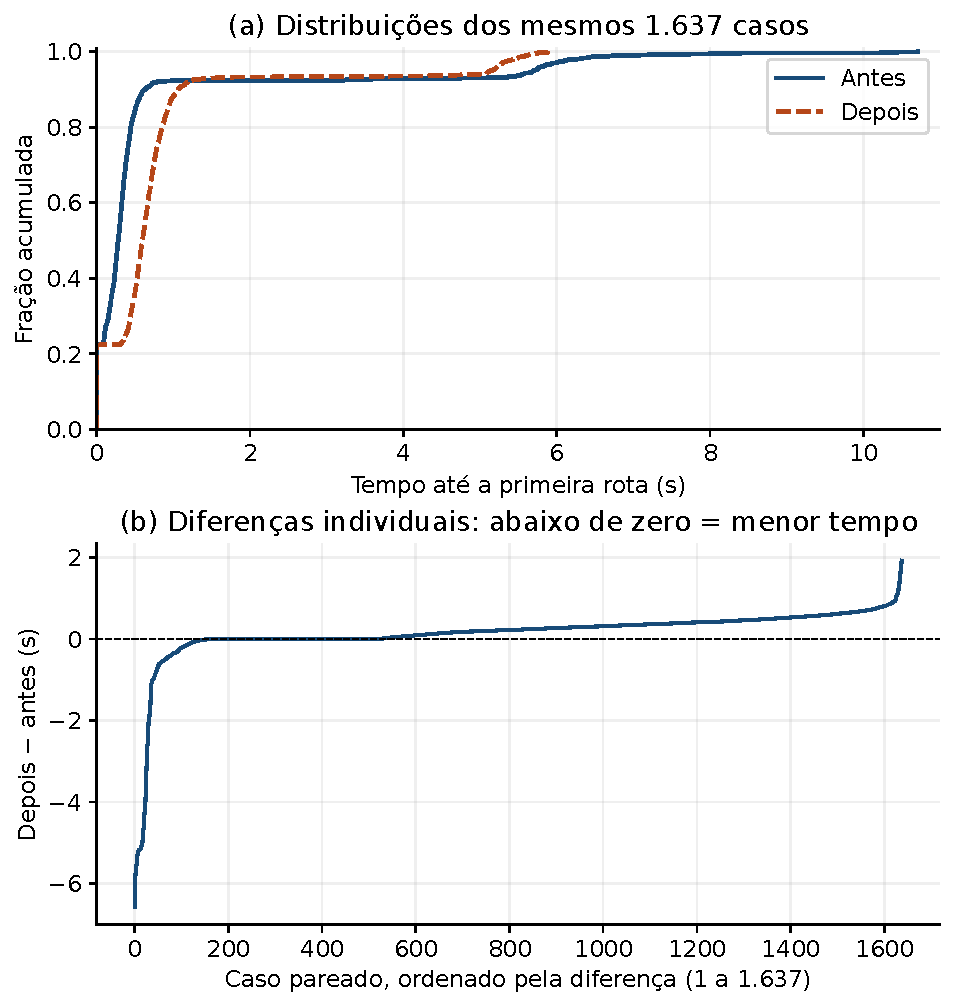
\includegraphics[width=\textwidth]{revisao-tecnico-cientifica-2026-11-02/benchmark-pareado.pdf}
\caption{Distribuições e diferenças das 1.637 medições pareadas até a primeira rota.}\label{fig:benchmark-pareado}
\fonte{CSV individual \nolinkurl{paired-results.csv}, ensaio de 1 nov. 2026; recálculo editorial em 2 nov. Cada diferença é depois menos antes para a mesma consulta; a ordenação não indica sequência temporal.}
\end{figure}
A Figura~\ref{fig:benchmark-pareado} utiliza todos os tempos individuais existentes, sem reconstrução de amostras a partir de médias ou percentis. O P95 segue o instrumento original: elemento ordenado de índice arredondado $0{,}95(n-1)$, com índice inicial zero. Os recortes por horário também mostram heterogeneidade: às 02h, o P95 aumentou de 0,739 para 1,281 s; às 08h, caiu de 5,760 para 5,215 s; às 14h, de 5,766 para 5,204 s. Não foram isolados efeitos de cache, carga, escalonamento ou concorrência; não se atribui causalidade a nenhum deles.
